\documentclass{article}
\usepackage[utf8]{inputenc}
\usepackage{ragged2e}
\usepackage{parskip}
\usepackage[T1]{fontenc}
\usepackage[utf8]{inputenc}
\usepackage[table]{xcolor}
\usepackage{graphicx}
\usepackage{mathtools}
\usepackage{glossaries}
\usepackage{float}
\usepackage{pgfplots}
\usepackage{multicol}
\usepackage{subcaption}
\usepackage{pdfpages}
\usepackage[margin=3cm]{geometry}
\usepackage{listings}
\usepackage{csvsimple}
\usepackage{rotating}
\usepackage[english]{babel}

\lstset{
  basicstyle=\footnotesize,
  breakatwhitespace=false,
  breaklines=true,
  extendedchars=true,
  frame=single,
  keepspaces=true,
  numbers=left,
  showstringspaces=true,
  tabsize=4,
  title=\lstname
}

\begin{document}
  \centering        
    \vfill
    
       {\LARGE \textbf{Travaux Pratiques : Gènes, génomes et alignement de séquences}} \\[1in]
    
    \justifying
     
  \section{Alignement de séquences (principes)}
  
  Au cours de l'évolution biologique, une séquence d'ADN change, le plus souvent en raison d'erreurs aléatoires dans la réplication ou la copie d'une séquence d'ADN. Ces erreurs de réplication sont appelées mutations. Les différents événements de mutation qui peuvent survenir sont:
  \begin{itemize}
  \item Des substitutions : où une base (ou un acide aminé, dans les séquences protéiques) est remplacée par une autre;
  \item Des insertions : lorsqu'une ou plusieurs bases contiguës sont insérées dans une séquence;
  \item Et des délétions : lorsqu'une ou plusieurs bases contiguës sont supprimées d'une séquence.
  \end{itemize}
  
L'objectif de l'alignement de séquences est, à partir de deux séquences, de générer une hypothèse sur les positions de séquences dérivées d'une position de séquence ancestrale commune. En pratique, nous développons cette hypothèse en alignant les séquences les unes sur les autres en insérant des gaps, si nécessaire, d'une manière qui maximise leur similarité. C'est une approche de parcimonie maximale, où nous supposons que l'explication la plus simple (celle impliquant le moins d'événements de mutation extrême) est la plus probable.

L'alignement de séquences sert, entre autres, à identifier des fonctions de proteines. Le rôle des proteines étant essentiel, on part du principe que deux proteines de séquenses similaires auront des propriété similaires. On peut donc rapprocher la séquence de proteines inconnues à celles connues et en déduire leur fonction.

On représente un alignement de la manière suivante :
\begin{center}
 AGCTGCTATGATACCGACGAT\\
A - - T - C - AT -ATACCGACGAT  
\end{center}



\section{Approche naïve}

Nous utiliserons une matrice d’identité, nous attribuons 1 point pour un match (même acide aminé) et 0 pour une substitution, une insertion/délétion.

Nous comparons deux séquences : \newline
Seq1 : ACCGGTGGAACCGGTAACACCCAC \\
Seq2 : ACCGGTAACCGGTTAACACCCAC

La première étape est de créer une matrice de substitution, voir page 2. La seconde étape est de combler cette matrice en suivant les directives indiquées (match=1, autre = 0).

\begin{center}
\begin{tabular}{|c|c|c|c|c|c|c|c|c|c|c|c|c|c|c|c|c|c|}
\hline
 &A&C&C&G&G&T&G&G&A&A&C&C&G&G&T&T&A\\
\hline
A&1&& & & & & & &1&1& & & & & & &1\\
\hline
C& &2& & & & & & & & & & & & & & &\\
\hline
C& & & & & & & & & & & & & & & & &\\
\hline
G& & & & & & & & & & & & & & & & &\\
\hline
G& & & & & & & & & & & & & & & & &\\
\hline
T& & & & & & & & & & & & & & & & &\\
\hline
A& & & & & & & & & & & & & & & & &\\
\hline
A& & & & & & & & & & & & & & & & &\\
\hline
C& & & & & & & & & & & & & & & & &\\
\hline
C& & & & & & & & & & & & & & & & &\\
\hline
G& & & & & & & & & & & & & & & & &\\
\hline
G& & & & & & & & & & & & & & & & &\\
\hline
T& & & & & & & & & & & & & & & & &\\
\hline
T& & & & & & & & & & & & & & & & &\\
\hline
A& & & & & & & & & & & & & & & & &\\
\hline
\end{tabular}
    \end{center}


La matrice se remplit de la façon suivante :
\begin{itemize}
\item On part de la case en haut à gauche.
\item Un déplacement en diagonal indique un match (+1)
\end{itemize}
 
Une fois remplie, nous cherchons les plus longs chemins. C’est à dire que nous cherchons les endroits dans la matrice qui maximisent les déplacements en diagonale. Il faut alors repérer les nombres les plus grands dans la matrice.

Une fois identifiés, nous partons de la case la plus en bas à droite de la diagonale et nous la remontons en arrière pour transcrire l'alignement en écrivant les caractères de chacune des deux séquences à chaque ligne et colonne correspondant à la diagonale que vous suivez.

Lorsque nous rencontrons une coupure dans la diagonale, nous trouvons la diagonale suivante la plus longue qui commence dans une cellule qui est en haut et/ou à gauche de la cellule actuelle.
\ 
Pour chaque déplacement vers le haut (non en diagonale), vous devez insérer un espace dans la séquence de l'axe horizontal de votre matrice. Pour chaque déplacement vers la gauche, insérez un espace dans la séquence de l'axe vertical de votre matrice.

\vfill
	\textbf{Exemple :}
    \begin{itemize}
    \item Déplacement en diagonal = les lettres se font face (match ou mismatch)
    \end{itemize}
\begin{center}
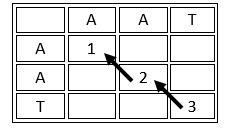
\includegraphics[]{figures/match.png}
\end{center}

Alignement :\\
AAT\\
AAT

\begin{itemize}
 \medbreak
\item Déplacement vers le haut = insertion d’un ‘-‘ dans la séquence horizontale.
\end{itemize}
\begin{center}
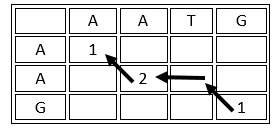
\includegraphics[]{figures/dep_haut.png}
\end{center}

Alignement :\\
AA-G\\
AATG

\begin{itemize}
\item Déplacement vers la droite = insertion d’un ‘-‘ dans la séquence verticale.
\end{itemize}
\begin{center}
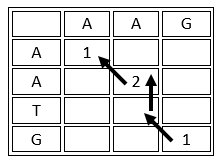
\includegraphics[]{figures/dep_droite.png}
\end{center}

Alignement :\\
AATG\\
AA-G
\medbreak

\textbf{Exercice 1 :}
\begin{itemize}
\item Remplissez la matrice page 2, vous pouvez juste indiquer les matchs dans la matrice.
\item Identifiez les plus longs chemins.
\item Ecrire le meilleur alignement.
\item La matrice utilisée est-elle la plus réaliste ? Justifiez.
\end{itemize}

\newpage
\section{Needleman-Wunch}
L'alignement que nous venons de construire était un alignement global naïf, ce qui signifie que nous alignons les deux séquences de leur début à leur fin. Saul B. Needleman et Christian D. Wunsch en 1970 ont publié un algorithme d’alignement global, moins naïf, que nous allons programmer sur Java. Leur algorithme divise le problème global d'alignement en une série de problèmes de taille inférieure.

Il est aussi connu sur les noms : \textit{optimal matching algorithm} et \textit{global alignment technique}.

\subsection{Principe}

Nous comparerons deux séquences :\\
Seq1 = ATCGAACCTG \\
Seq2 = ATGAATG
\medbreak

a) Définition du coût des différents événements :
\begin{itemize}
\item Match = 3
\item Mismatch = -1
\item Indel (insertion ou delétion)= -2
\end{itemize}

%\newline
\medbreak
\textbf {Exercice 2 :}
\begin{itemize}
\item Créez un package \textbf{align} dans Eclipse.
\item Créez une nouvelle classe \textbf{alignement}.
\item Importez le package \textbf{java.util.Arrays}.
\item Créez trois variables static correspondant aux match, mismatch et indel.
\item Attribuez-leur les valeurs correspondantes.
\item Créer votre \textbf{main} de la façon suivante :
\end{itemize}

\begin{lstlisting}{Java}
public static void main(String[] args){
	 String S = "ATCGAACCTG";
	 String T = "ATGAATG";
} 
\end{lstlisting}

b)  Création de la matrice.

Contrairement à la matrice naïve les matrices de Needleman-Wunch contiennent une ligne et colone dites d'initialisation.

Caractéristiques de la matrice :
\begin{itemize}
\item Nombre colonne = Taille(seq1)+1
\item Nombre ligne = Taille(seq2)+1
\end{itemize}


\begin{center}
\begin{tabular}{|c|c|c|c|c|c|c|c|c|c|c|c|}
\hline
 &&A&T&C&G&A&A&C&C&T&G\\
\hline
 & & & & & & & & & & & \\
\hline
A& & & & & & & & & & & \\
\hline
T& & & & & & & & & & & \\
\hline
G& & & & & & & & & & & \\
\hline
A& & & & & & & & & & & \\
\hline
A& & & & & & & & & & & \\
\hline
T& & & & & & & & & & & \\
\hline
G& & & & & & & & & & & \\
\hline
\end{tabular}
\end{center}
\medbreak
\textbf{Exercice 3 :} 

Créer une fonction \textbf{initmatrix} qui construit une matrice comme ci-dessus.
\begin{lstlisting}{Java}
public static int[][] initMatrix(String S, String T) {
	 //code de creation d'une matrice
	 return matrix;
 }
\end{lstlisting}

c) Initialisation la matrice :
\begin{center}
\begin{tabular}{|c|c|c|c|c|c|c|c|c|c|c|c|}
\hline
 &&A&T&C&G&A&A&C&C&T&G\\
\hline
&0&-2& & & & & & & & & \\
\hline
A&-2& & & & & & & & & & \\
\hline
T& & & & & & & & & & & \\
\hline
G& & & & & & & & & & & \\
\hline
A& & & & & & & & & & & \\
\hline
A& & & & & & & & & & & \\
\hline
T& & & & & & & & & & & \\
\hline
G& & & & & & & & & & & \\
\hline
\end{tabular}
    \end{center}
    \medbreak
    
\textbf{Exerice 4 :}
\begin{itemize}
\item Remplir la première ligne et première colonne à la main
\item Créer une fonction \textbf{initglobal} qui permet de compléter la première ligne et la première colonne comme vous l’avez fait à la main ci-dessus.
\end{itemize}

\begin{lstlisting}{Java}
//fonction qui ininite la premiere colonne et ligne
public static int[][] initGlobal( int[][] matrix) {
		//calcul de la premiere ligne
		//calcul de la premiere colonne
	return matrix;
	}
\end{lstlisting}
\newpage

d) Remplissage la matrice :
\begin{center}
\begin{tabular}{|c|c|c|c|c|c|c|c|c|c|c|c|}
\hline
 &&A&T&C&G&A&A&C&C&T&G\\
\hline
&0&-2& & & & & & & & & \\
\hline
A&-2&\textbf{3}& & & & & & & & & \\
\hline
T& & & & & & & & & & & \\
\hline
G& & & & & & & & & & & \\
\hline
A& & & & & & & & & & & \\
\hline
A& & & & & & & & & & & \\
\hline
T& & & & & & & & & & & \\
\hline
G& & & & & & & & & & & \\
\hline
\end{tabular}
    \end{center}
    
    
\textbf{Exerice 5 :}
\begin{itemize}
\item Remplir la matrice à la main. Pour chaque case pointer à l’aide d’une flèche la case à partir de laquelle le calcul a été fait (voir exemple si dessus). Attention : pour remplir une case il est nécessaire de connaitre les 3 cases pouvant la précéder.
\item Coder la fonction \textbf{max3} qui compare trois scores et retourne le plus élevé et qui identifiera le score maximum entre un déplacement en diagonale, vers le bas ou vers la droite.
\begin{lstlisting}{Java}
 public static int max3(int a, int b, int c){
	 // comparaison entre trois valeurs et retourne la plus elevee
	 }
\end{lstlisting}

\item Coder la fonction \textbf{score} qui permettra de savoir si le déplacement en diagonale est un match ou un mismatch et de retourner le score
\begin{lstlisting}{Java}
public static int score(char s,char t) {
 	// votre code de comparaison pour savoir s'il s'agit d'un match ou mismatch
 	}
\end{lstlisting}

\item Coder la fonction \textbf{fillNW} qui permet de remplir la matrice et renvoi l'élément trouvé dans la case la plus en bas à droite, en utilisant : \textbf{max3} et \textbf{score} \\


\begin{lstlisting}{Java}
public static int fillNW(int[][] matrix, String S, String T) { 
	for (int i=1; i<=S.length();i++ ) {
		for (int j=1; j<=T.length();j++) {
			//calcul du meilleur score pour la case matrix[i][j]
			}
		}
	return matrix[S.length()][T.length()];
	}
\end{lstlisting}
\end{itemize}
\newpage

e) Détection du meilleur alignement.

Pour déterminer le meilleur alignement, on part de la case la plus bas à droite, on suit ensuite les flèches pour remonter la matrice, tout en retranscrivant l’alignement. 

\medbreak
\textbf{Exercice 6 :}
\begin{itemize}
\item Déterminer le meilleur alignement à la main.
\item Que fait la fonction \textbf{whichmax3} ?
\item A quoi correspondent a,b,c ?
\end{itemize}
\medbreak
\begin{lstlisting}{Java}
public static int whichMax3(int a, int b, int c) {
	if (a>b) {
		if (a>c) {return 1;}
		else {return 3;}
		}
	else {
		if (b>c) {return 2;}
		else {return 3;}
		}
	}
\end{lstlisting}

\begin{itemize}
\item Compléter la fonction \textbf{GetAln}, qui va chercher et afficher le meilleur alignement global.
\item Vous afficherez l'alignement selon le modèle suivant : \\
\end{itemize}
\begin{center}
\begin{tabular}{|c|c|c|c|c|}
\hline
Sequence&match&mismatch&gap S&gap T\\
\hline
S&T&A&T&-\\
\hline
matching&|&.& & \\
\hline
T&T&C&-&G\\
\hline
\end{tabular}
    \end{center}

\begin{lstlisting}{Java}
public static void getAln(int[][] matrix, String S, String T) {
	String alS="";
	String alT="";
	String matching="";
	int i =S.length();
	int j = T.length();
	
	while (i>0 & j>0) {
		int coming=whichMax3(matrix[i-1][j]+INDEL,matrix[i][j-1]+INDEL,matrix[i-1][j-1]+score(S.charAt(i-1),T.charAt(j-1)));
		if (coming==3) {
            //Actualiser als,alT et matching
		}
		else if (coming==1) {
    		//Actualiser als,alT et matching
		}
		else {
    		//Actualiser als,alT et matching
		}
	}
	
    //commentaire : gap dans T si T>S
	while (i>0) {
		alT=T.charAt(j-1)+alT;
		alS="-"+alS;
		j=j-1;
		matching=" "+matching;
	}
	
    //commentaire : gap dans S si S>T
	while (j>0) {
		alT=T.charAt(j-1)+alT;
		alS="-"+alS;
		j=j-1;
		matching=" "+matching;
	}
	//imprimer alS, matching et alT
}
\end{lstlisting}

\textbf{Exercice 7 :} 

Compléter le \textbf{main} et réaliser l'alignement de S et T.

\textbf{Exercice bonus :} 

Coder une fonction \textbf{printMatrix} qui réalise une sortie graphique de la matrice.

 \end{document}
